% $Header: /cvsroot/latex-beamer/latex-beamer/examples/beamerexample5.tex,v 1.22 2004/10/08 14:02:33 tantau Exp $

\documentclass[11pt]{beamer}

\usetheme{Darmstadt}

\usepackage{times}
\usefonttheme{structurebold}

%\usepackage[english]{babel}
\usepackage[portuges]{babel}
\usepackage{pgf,pgfarrows,pgfnodes,pgfautomata,pgfheaps}
\usepackage{amsmath,amssymb}
%\usepackage[latin8]{inputenc}
\usepackage[utf8]{inputenc}
\usepackage{graphicx}

\setbeamercovered{dynamic}

\newcommand{\Lang}[1]{\operatorname{\text{\textsc{#1}}}}

\newcommand{\Class}[1]{\operatorname{\mathchoice
  {\text{\sf \small #1}}
  {\text{\sf \small #1}}
  {\text{\sf #1}}
  {\text{\sf #1}}}}

\newcommand{\NumSAT}      {\text{\small\#SAT}}
\newcommand{\NumA}        {\#_{\!A}}

\newcommand{\barA}        {\,\bar{\!A}}

\newcommand{\Nat}{\mathbb{N}}
\newcommand{\Set}[1]{\{#1\}}

\pgfdeclaremask{tu}{beamer-tu-logo-mask}
\pgfdeclaremask{computer}{beamer-computer-mask}
\pgfdeclareimage[interpolate=true,mask=computer,height=2cm]{computerimage}{beamer-computer}
\pgfdeclareimage[interpolate=true,mask=computer,height=2cm]{computerworkingimage}{beamer-computerred}
\pgfdeclareimage[mask=tu,height=.5cm]{logo}{logounesp}

\logo{\pgfuseimage{logo}}

\title{Revisão Matemática: Números Complexos}
\author{Ney Lemke}
\institute[IBB-UNESP]{%
    Mec\^anica Qu\^antica }
%%%%%    Departamento de F\~AƒÂƒ\~A‚­sica e Biof\~AƒÂƒ\~A‚­sica}
\date{2012}                                

\colorlet{redshaded}{red!25!bg}
\colorlet{shaded}{black!25!bg}
\colorlet{shadedshaded}{black!10!bg}
\colorlet{blackshaded}{black!40!bg}

\colorlet{darkred}{red!80!black}
\colorlet{darkblue}{blue!80!black}
\colorlet{darkgreen}{green!80!black}

\def\radius{0.96cm}
\def\innerradius{0.85cm}

\def\softness{0.4}
\definecolor{softred}{rgb}{1,\softness,\softness}
\definecolor{softgreen}{rgb}{\softness,1,\softness}
\definecolor{softblue}{rgb}{\softness,\softness,1}

\definecolor{softrg}{rgb}{1,1,\softness}
\definecolor{softrb}{rgb}{1,\softness,1}
\definecolor{softgb}{rgb}{\softness,1,1}

\newcommand{\Bandshaded}[2]{
  \color{shadedshaded}
  \pgfmoveto{\pgfxy(-0.5,0)}
  \pgflineto{\pgfxy(-0.6,0.1)}
  \pgflineto{\pgfxy(-0.4,0.2)}
  \pgflineto{\pgfxy(-0.6,0.3)}
  \pgflineto{\pgfxy(-0.4,0.4)}
  \pgflineto{\pgfxy(-0.5,0.5)}
  \pgflineto{\pgfxy(4,0.5)}
  \pgflineto{\pgfxy(4.1,0.4)}
  \pgflineto{\pgfxy(3.9,0.3)}
  \pgflineto{\pgfxy(4.1,0.2)}
  \pgflineto{\pgfxy(3.9,0.1)}
  \pgflineto{\pgfxy(4,0)}
  \pgfclosepath
  \pgffill

  \color{black}  
  \pgfputat{\pgfxy(0,0.7)}{\pgfbox[left,base]{#1}}
  \pgfputat{\pgfxy(0,-0.1)}{\pgfbox[left,top]{#2}}
}

\newcommand{\Band}[2]{
  \color{shaded}
  \pgfmoveto{\pgfxy(-0.5,0)}
  \pgflineto{\pgfxy(-0.6,0.1)}
  \pgflineto{\pgfxy(-0.4,0.2)}
  \pgflineto{\pgfxy(-0.6,0.3)}
  \pgflineto{\pgfxy(-0.4,0.4)}
  \pgflineto{\pgfxy(-0.5,0.5)}
  \pgflineto{\pgfxy(4,0.5)}
  \pgflineto{\pgfxy(4.1,0.4)}
  \pgflineto{\pgfxy(3.9,0.3)}
  \pgflineto{\pgfxy(4.1,0.2)}
  \pgflineto{\pgfxy(3.9,0.1)}
  \pgflineto{\pgfxy(4,0)}
  \pgfclosepath
  \pgffill

  \color{black}  
  \pgfputat{\pgfxy(0,0.7)}{\pgfbox[left,base]{#1}}
  \pgfputat{\pgfxy(0,-0.1)}{\pgfbox[left,top]{#2}}
}

\newcommand{\BaenderNormal}
{%
  \pgfsetlinewidth{0.4pt}
  \color{black}
  \pgfputat{\pgfxy(0,5)}{\Band{input tapes}{}}
  \pgfputat{\pgfxy(0.35,4.6)}{\pgfbox[center,base]{$\vdots$}}
  \pgfputat{\pgfxy(0,4)}{\Band{}{}}

  \pgfxyline(0,5)(0,5.5)
  \pgfxyline(1.2,5)(1.2,5.5)
  \pgfputat{\pgfxy(0.25,5.25)}{\pgfbox[left,center]{$w_1$}}

  \pgfxyline(0,4)(0,4.5)
  \pgfxyline(1.8,4)(1.8,4.5)        
  \pgfputat{\pgfxy(0.25,4.25)}{\pgfbox[left,center]{$w_n$}}
  \ignorespaces}

\newcommand{\BaenderZweiNormal}
{%
  \pgfsetlinewidth{0.4pt}
  \color{black}
  \pgfputat{\pgfxy(0,5)}{\Band{Zwei Eingabeb\~AƒÂƒ\~A‚¤nder}{}}
  \pgfputat{\pgfxy(0,4.25)}{\Band{}{}}

  \pgfxyline(0,5)(0,5.5)
  \pgfxyline(1.2,5)(1.2,5.5)
  \pgfputat{\pgfxy(0.25,5.25)}{\pgfbox[left,center]{$u$}}

  \pgfxyline(0,4.25)(0,4.75)
  \pgfxyline(1.8,4.25)(1.8,4.75)        
  \pgfputat{\pgfxy(0.25,4.5)}{\pgfbox[left,center]{$v$}}
  \ignorespaces}

\newcommand{\BaenderHell}
{%
  \pgfsetlinewidth{0.4pt}
  \color{black}
  \pgfputat{\pgfxy(0,5)}{\Bandshaded{input tapes}{}}
  \color{shaded}
  \pgfputat{\pgfxy(0.35,4.6)}{\pgfbox[center,base]{$\vdots$}}
  \pgfputat{\pgfxy(0,4)}{\Bandshaded{}{}}

  \color{blackshaded}
  \pgfxyline(0,5)(0,5.5)
  \pgfxyline(1.2,5)(1.2,5.5)
  \pgfputat{\pgfxy(0.25,5.25)}{\pgfbox[left,center]{$w_1$}}

  \pgfxyline(0,4)(0,4.5)
  \pgfxyline(1.8,4)(1.8,4.5)        
  \pgfputat{\pgfxy(0.25,4.25)}{\pgfbox[left,center]{$w_n$}}
  \ignorespaces}

\newcommand{\BaenderZweiHell}
{%
  \pgfsetlinewidth{0.4pt}
  \color{black}
  \pgfputat{\pgfxy(0,5)}{\Bandshaded{Zwei Eingabeb\~AƒÂƒ\~A‚¤nder}{}}%
  \color{blackshaded}
  \pgfputat{\pgfxy(0,4.25)}{\Bandshaded{}{}}
  \pgfputat{\pgfxy(0.25,4.5)}{\pgfbox[left,center]{$v$}}
  \pgfputat{\pgfxy(0.25,5.25)}{\pgfbox[left,center]{$u$}}%

  \pgfxyline(0,5)(0,5.5)
  \pgfxyline(1.2,5)(1.2,5.5)

  \pgfxyline(0,4.25)(0,4.75)
  \pgfxyline(1.8,4.25)(1.8,4.75)        
  \ignorespaces}

\newcommand{\Slot}[1]{%
  \begin{pgftranslate}{\pgfpoint{#1}{0pt}}%
    \pgfsetlinewidth{0.6pt}%
    \color{structure}%
    \pgfmoveto{\pgfxy(-0.1,5.5)}%
    \pgfbezier{\pgfxy(-0.1,5.55)}{\pgfxy(-0.05,5.6)}{\pgfxy(0,5.6)}%
    \pgfbezier{\pgfxy(0.05,5.6)}{\pgfxy(0.1,5.55)}{\pgfxy(0.1,5.5)}%
    \pgflineto{\pgfxy(0.1,4.0)}%
    \pgfbezier{\pgfxy(0.1,3.95)}{\pgfxy(0.05,3.9)}{\pgfxy(0,3.9)}%
    \pgfbezier{\pgfxy(-0.05,3.9)}{\pgfxy(-0.1,3.95)}{\pgfxy(-0.1,4.0)}%
    \pgfclosepath%
    \pgfstroke%
  \end{pgftranslate}\ignorespaces}

\newcommand{\SlotZwei}[1]{%
  \begin{pgftranslate}{\pgfpoint{#1}{0pt}}%
    \pgfsetlinewidth{0.6pt}%
    \color{structure}%
    \pgfmoveto{\pgfxy(-0.1,5.5)}%
    \pgfbezier{\pgfxy(-0.1,5.55)}{\pgfxy(-0.05,5.6)}{\pgfxy(0,5.6)}%
    \pgfbezier{\pgfxy(0.05,5.6)}{\pgfxy(0.1,5.55)}{\pgfxy(0.1,5.5)}%
    \pgflineto{\pgfxy(0.1,4.25)}%
    \pgfbezier{\pgfxy(0.1,4.25)}{\pgfxy(0.05,4.15)}{\pgfxy(0,4.15)}%
    \pgfbezier{\pgfxy(-0.05,4.15)}{\pgfxy(-0.1,4.2)}{\pgfxy(-0.1,4.25)}%
    \pgfclosepath%
    \pgfstroke%
  \end{pgftranslate}\ignorespaces}

\newcommand{\ClipSlot}[1]{%
  \pgfrect[clip]{\pgfrelative{\pgfxy(-0.1,0)}{\pgfpoint{#1}{4cm}}}{\pgfxy(0.2,1.5)}\ignorespaces}

\newcommand{\ClipSlotZwei}[1]{%
  \pgfrect[clip]{\pgfrelative{\pgfxy(-0.1,0)}{\pgfpoint{#1}{4.25cm}}}{\pgfxy(0.2,1.25)}\ignorespaces}


\AtBeginSection[]{\frame{\frametitle{Outline}\tableofcontents[current]}}

\begin{document}

\frame{\titlepage}

%\section*{Outline}

\frame{\frametitle{Outline}\tableofcontents} 

\frame{\frametitle{Bibliografia}
  \begin{itemize}
  \item ``Física Matemática'', E. Butkov, Ed. LTC, 1$^a$ Edição, 1988.
  \item ``An Imaginary Tale: The history of $\sqrt{-1}$'',
    P. J. Nahin, Princeton University Press, 1998. 
  \end{itemize}


}
\section{Introdução}
\frame{\frametitle{Equação Cúbia}

Considere uma equação cúbica na forma:

$$x^3 +p x = q$$

del Ferro (1465-1526) propôs:

$$x=u+v$$
}
   
\frame{\frametitle{Equação Cúbica}
Neste caso temos:

$$u^3+v^3+(3 uv +p)(u+v)=q$$

Escolhendo:

$$3u v+p=0$$

Temos:

$$u^3+v^3=q$$
}
\frame{\frametitle{Equação Cúbica}
Essa equações podem ser escritas como:

$$u^6-qu^3-\frac{p^3}{27}=0$$

Nos restringindo apenas a raiz positiva:

$$u^3=\frac{q}{2}+\sqrt{\frac{q^2}{4}+\frac{p^3}{27}} \quad v^3=\frac{q}{2}+\sqrt{\frac{q^2}{4}-\frac{p^3}{27}}$$

Finalmente:

$$x=\sqrt[3]{\frac{q}{2}+\sqrt{\frac{q^2}{4}+\frac{p^3}{27}}} +\sqrt[3]{\frac{q}{2}+\sqrt{\frac{q^2}{4}-\frac{p^3}{27}}}$$
}

\frame{\frametitle{Equação Cúbica}
O que ocorre se:

$$\frac{q^2}{4}-\frac{p^3}{27}<0$$

Neste caso teremos que manipular raízes de números complexos. 
O que violava o fato evidente que esses números não 
existem. 

Solução de Cardano (1501-1576) foi assumir que essas aberrações
exisitiam e tratá-las como se fossem números. 
}

\frame{\frametitle{Surgimento dos Números Complexos}
  \begin{itemize}
  \item Descartes
  \item Argand
  \item Euler
  \item Gauss
  \item Riemann
  \end{itemize}
}

\frame{\frametitle{Números complexos: fato ou mito}
  \begin{itemize}
  \item Os números complexos tornam a álgebra mais simples.
  \item Extendem o conceito de número, mas existem outras possibilidades:
    \begin{itemize}
    \item Quartenions
    \item Números Perplexos 
    \end{itemize}
\item A função de onda é uma função complexa. Ou seja eles podem ser
  essenciais para compreender nossa realidade física. 
\end{itemize}
}
\section{Operações Matemáticas}
\frame{\frametitle{Operações Fundamentais}
O conjunto dos números complexos $\mathbb{C}$ satisfaz as
propriedades:

\begin{itemize}
\item Se $z\in \mathbb{C}$ então $z=x+iy$. Onde $x,y\in \mathbb{R}$ e $i^2=-1$.
\item $z_1+z_2=(x_1+x_2)+(y_1+y_2)i$
\item $z_1 z_2=(x_1x_2 -y_1y_2)+(x_1y_2+x_2x_1)i$
\item $z^*=\overline{z}=x-iy$
\item $|z|^2=x^2+y^2$
\end{itemize}
}

\frame{\frametitle{Divisão}

Sejam $z_1$ e $z_2\in\mathbb{C}$. 

$$\frac{z_1}{z_2}=\frac{z_1\overline{z_2}}{z_2\overline{z_2}}=\frac{z_1\overline{z_2}}{|z_2|^2}$$
}

\section{Representação Gráfica}

\frame{\frametitle{Plano de Argand}

  \begin{minipage}{5cm}
\begin{center}
\includegraphics[scale=0.1]{argand.png}
\end{center}
  \end{minipage}
  \begin{minipage}{5cm}
Fórmula de de Moivre

$$z=r (\cos \varphi + i\sin \varphi)$$ 

onde $r=|z|$
  \end{minipage}
}

\frame{\frametitle{Fórmula de Euler}

$$z=r(\cos \varphi+ i\sin\varphi)=re^{i\varphi}$$

$r$ é o módulo e $\varphi$ a fase do número complexo. 

Mostre que:

$$\overline{e^{i\varphi}}=e^{-i\varphi}$$
}

\frame{\frametitle{Interpretação das Operações}
  \begin{itemize}
  \item Soma de números Complexos é equivalente a soma de dois vetores.
  \item Multiplicação por números complexos é equivalente a:
    \begin{description}
    \item[número real positivo] é equivalente a uma mudança de escala
    \item[$r$=1] é equivalente a rotação por um ângulo $\varphi$
    \end{description}
  \end{itemize}
}

\section{Resultados Matematicos}

\frame{\frametitle{Partes reais e Imaginária}
Seja $z\in\mathbb{C} $ e $ z=x+iy$ 
\begin{description}
\item[Parte Real] $\Re (z)=x=\frac{z+\overline{z}}{2}$
\item[Parte Imaginária] $\Im (z) =y=\frac{z-\overline{z}}{2 i}$
\end{description}
}

\frame{\frametitle{$n$-ésima raiz da unidade}

Encontre todas as soluções da equação:

$$z^n=1$$


}

\frame{\frametitle{Fórmulas trigonométricas}
Usando a fórmula de Euler mostre que:

$$\cos \alpha\cos\beta=\frac{1}{2} \left[ \cos (\alpha+\beta) + \cos
  (\alpha -\beta )\right]$$

Calcule também:
\begin{enumerate}
\item $$\sum_{n=0}^\infty \frac{\cos n\theta}{2^n}$$
\item $$\sum_{n=1}^\infty \frac{\cos n\theta}{2^nn}$$
\end{enumerate}
}

\frame{\frametitle{Funções Complexas}

Toda função real possui uma função complexa equivalente. Por exemplo 

$$\cos z=\frac{e^{iz}+e^{-iz}}{2}=\frac{e^{i(x+iy)}+e^{-i(x+iy})}{2}=\frac{e^{ix-y}+e^{-ix+y}}{2}$$

As regras de derivação e integração são as mesmas para funções reais e complexas. 

}

\frame{\frametitle{Integração: Cauchy Riemann}

Existe um resultado importante para funções complexas que é muito
explorado na matemática. A integral fechada de uma função analítica 
é sempre nula. 

$$\oint f(z)dz =0$$
}

\frame{\frametitle{Integração}

Calcule a integral:

$$\oint_C \frac{dz}{z}$$

onde $C$ é um círculo de raio $r$ em torno da origem. 

Dica: Use a equação de Euler. 
}

\end{document}


\frame{\frametitle{Espaço Vetorial} Formalmente definimos vetor como
  sendo um elemento de um espaço vetorial.

  Um espaço vetorial é um conjunto que possui duas operações, chamadas
  de soma e multiplicação por escalar. Estas operações obedecem estas
  propriedades:

  \begin{enumerate}
  \item $\vec{x}+\vec{y}=\vec{y}+\vec{x}$
  \item $(\vec{x}+\vec{y})+\vec{z}=\vec{x}+(\vec{y}+\vec{z})$
  \item $\vec{x}+0=\vec{x}$
  \item $\forall \vec{x} \exists \vec{y}\quad  \mbox{tq} \quad \vec{x}+\vec{y}=0$
  \end{enumerate}
}

\frame{\frametitle{Espaço Vetorial} Sejam $\alpha$ e $\beta$
  quantidades escalares:
  \begin{enumerate}
  \item $\alpha (\beta \vec{x})=(\alpha \beta)\vec{x}$
  \item $(\alpha+\beta)\vec{x}=\alpha\vec{x}+\beta\vec{x}$
  \item $\alpha(\vec{x}+\vec{y})=\alpha\vec{x}+\alpha\vec{y}$
  \end{enumerate}
}

\frame{\frametitle{Exercício} Mostre que os números complexos formam
  um espaço vetorial, se considerarmos multiplicação por escalar,
  multiplicação por real.

}

\frame{\frametitle{Combinação Linear}

$$\alpha_i \vec{x_i}+\ldots+\alpha_n \vec{x_n}=\sum_{i=1}^n \alpha_i\vec{x}_i$$

}

\frame{\frametitle{Vetores linearmente independentes}

  $n$ vetores são considerados linearmente independentes se e somente
  se:
$$\sum_{i=1}^n \alpha_i\vec{x}_i=0$$
implicar que $\forall i \quad \alpha_i=0$.  }

\frame{\frametitle{Subespaço Vetorial}

  Considere $k$ vetores $\vec{x}_i, \ldots ,\vec{x}_k$ e o conjunto de
  vetores na forma:

$$\vec{y}=\sum_{i=1}^k \alpha_i \vec{x_i}$$

Este conjunto é chamado de sub-espaço vetorial. Observe que este
conjunto é um espaço vetorial.  }


\frame{\frametitle{Subespaço Vetorial} Se os vetores $\vec{x}_i,
  \ldots ,\vec{x}_k$ forem linearmente independentes dizemos que eles
  formam uma base para o sub-espaço vetorial. Se $k$ for a
  dimensionalidade do espaço dizemos que o conjunto é uma base para o
  espaço vetorial. 
}

\frame{\frametitle{Subespaço Vetorial} 
Suponha que os vetores $\vec{e}_i $ sejam uma base para um espaço vetorial,
ou seja 
$$\vec{x}=\sum_{i=1}^n x_i \vec{e}_i$$

Representamos o vetor usando o vetor coluna:
$$\vec{x}=\begin{pmatrix} x_1 \\ \ldots \\ x_n \end{pmatrix}$$
}

\frame{\frametitle{Operadores} 

Um operador é uma função que associa um elemento do espaço vetorial a outro 
elemento do espaço vetorial:

$$\vec{y}=F(\vec{x})$$

}


\frame{\frametitle{Operador Linear} 
Um operador Linear deve satisfazer asseguintes condições:

\begin{enumerate}
\item $L(\alpha \vec{x})=\alpha L\vec{x}$
\item $L(\vec{x}+\vec{y})=L\vec{x}+L\vec{y}$
\item $L(0)=0$
\end{enumerate}


}
\frame{\frametitle{Operador Linear} 
$$L(\vec{e}_i)=\vec{a}_i=\sum_{j=1}^n a_{ji}\vec{e}_j$$

$$\vec{y}=L\vec{x}$$
$$\vec{y}=L\sum_{i=1}^n x_i \vec{e}_i=\sum_{ij} x_i  a_{ji}\vec{e}_j$$
$$y_k=\sum_{i}a_{ki} x_i$$
}

\frame{\frametitle{Composição de Operadores Lineares} 

$$\vec{y}=A \vec{x} \quad \vec{z}=B\vec{y} \quad \vec{z}=C\vec{x}$$

$$y_i=\sum_ja_{ij}x_j\quad z_k=\sum_jb_{ki}y_i  $$

$$z_k=\sum_{ij}a_{ij}b_{ki}x_j$$

$$c_{kj}=\sum_i b_{ki} a_{ij}$$
}

\frame{\frametitle{Exemplos de Operadores Lineares} 
  \begin{itemize}
  \item $I$: $I\vec{x}=\vec{x}$
  \item $N$: $N\vec{x}=-\vec{x}$
  \item Rotação
  \end{itemize}
}

\frame{\frametitle{Mudança de Base} 

$$\vec{x}=\sum_i x_i \vec{e}_i \quad \vec{x}=\sum_i x_i^\prime \vec{g}_i$$

$$\vec{g}=\sum_j g_{ji}\vec{e}_j\quad G=[ g_{ij}]$$
$$\vec{e}_j=\sum_it_{ij}\vec{g}_i\quad T=[ t_{ij}]$$

$$\vec{x}=\sum_jx_j\vec{e}_j=\sum_{ji}x_jt_{ij}\vec{g}_i=\sum_i \vec{g}_i \sum_j t_{ij} x_j$$

$$x_i^\prime=\sum_j t_{ij} x_j$$
$$x_i=\sum_j g_{ij} x_j$$
}

\frame{\frametitle{Mudança de Base} 
$$\vec{x}=G\vec{x^\prime}$$
$$\vec{x^\prime}=T\vec{x}$$
$$\vec{x}=TG\vec{x}$$
$$TG=I$$
}

\frame{\frametitle{Mudança de Base} 
$$\vec{y}=A \vec{x} \quad \vec{y^\prime}= A^\prime \vec{x^\prime}$$
$$\vec{y^\prime}=T\vec{y} \quad \vec{x^\prime}=T\vec{x}$$
$$T\vec{y}=A^\prime T\vec{x}$$
$$\vec{y}=T^{-1}A^\prime T\vec{x}$$
$$A=T^{-1}A^\prime T$$
$$A^\prime=TA T^{-1}$$
}



\frame{\frametitle{Matriz Transposta}
Seja uma matriz:

$$A=[A_{ij}]$$


a matriz transposta $A^T$ é dada por:

$$A^T_{ij}=A_{ji}$$

}
\frame{\frametitle{Determinantes} 

\underline{Definição} O determinante de uma matriz quadrada é definido por:

$$\det A =\sum_{\sigma\in S_n}\mbox{sgn} (\sigma)\prod_{i=1}^n A_{i,\sigma_i}$$

a soma é calculada sobre todas as permutações $\sigma$ , o sinal de uma permutação está relacionado 
ao número de trocas a partir da seq. ordenada $\{1,\ldots , n\}$, se o número de trocas for par 
o sinal é positivo e negativo caso contrário. 

 } 


\frame{\frametitle{Determinantes} 
\underline{Propriedades}

\begin{enumerate}
\item $\det AB= \det A \det B$
\item $det A^T=\det A$
\item $det (\alpha A) = \alpha^n det A$
\item $\det I$=1
\item $det T^{-1}=1/(det T)$
\item $det TAT^{-1}=det A$
\end{enumerate}
}

\frame{\frametitle{Traço} 

O Traço de uma matriz quadrada e dado por:

$$\mbox{Tr} A=\sum_{i=1}^n A_{ii}$$

\underline{Propriedades}
\begin{enumerate}
\item $\mbox{Tr} A^T=\mbox{Tr} A$
\item $\mbox{Tr} (A+B)=\mbox{Tr} A+ \mbox{Tr} B$
\item $\mbox{Tr} AB= \mbox{Tr} BA$  (propriedade circular)
\item $\mbox{Tr} TAT^{-1} = \mbox{Tr} A$ (Traços são invariantes a mudanças de base)
\end{enumerate}
}

\frame{\frametitle{Produto Interno}
O produto interno é um escalar $(\vec{x},\vec{y})$ obtido a partir de dois vetores $\vec{x}$ 
e $\vec{y}$ e que satisfaz as propriedades:

\vspace{1 cm}


  \begin{minipage}{5cm}
\centering{Espaço Reais}

    \begin{itemize}
\item $(\vec{x},\vec{y})=(\vec{y},\vec{x})$
\item $(\vec{x},\vec{y}+\vec{z})=(\vec{x},\vec{y})+(\vec{x},\vec{z})$
\item $(\vec{x},\vec{x})\geq 0$
    \end{itemize}
  \end{minipage}
  \begin{minipage}{5cm}
\centering{Espaço Complexos}

    \begin{itemize}
\item $(\vec{x},\vec{y})=\overline{(\vec{y},\vec{x})}$
\item $(\vec{x},\vec{y}+\vec{z})=(\vec{x},\vec{y})+(\vec{x},\vec{z})$
\item $(\vec{x},\vec{x})\geq 0$
    \end{itemize}
  \end{minipage}
\vspace{1 cm}
$(\vec{x},\vec{x} )$ é denominado a norma do vetor. 
} 

\frame{\frametitle{Produto Interno}
  \begin{minipage}{5cm}
\centering{Espaço Reais}
    \begin{itemize}
\item $(\vec{x},\vec{y} )=\sum_{i=1}^n x_i y_i=\vec{x}^T\vec{y}$
    \end{itemize}
  \end{minipage}
  \begin{minipage}{5cm}
\centering{Espaço Complexos}
    \begin{itemize}
\item $(\vec{x},\vec{y} )=\sum_{i=1}^n x_i^* y_i=\vec{x}^\dagger\vec{y}$
    \end{itemize}
  \end{minipage}
\vspace{1 cm}

$A^\dagger$ é a matriz transposta e conjugada de $A$. Lê-se {\it dagger} ou adaga. 
} 


\frame{\frametitle{Base ortonormal}
Dois vetores são ditos ortogonais se:

$$(\vec{x},\vec{y})=0$$

Uma base é dita ortonormal se:

$$(\vec{e}_i,\vec{e}_j)=\delta_{ij}$$

}

\frame{\frametitle{Classes de Matrizes}
  \begin{description}
  \item[Unitárias] $U^\dagger U=I$
  \item[Ortogonais] $G^T G=I$
  \item[Hermitianas] $G^\dagger=G$
  \end{description}
}

\frame{\frametitle{Autovalores e Autovetores}
$$A\vec{x}=\lambda \vec{x}$$

$\vec{x}$ é um autovetor

$\lambda$ é um autovalor

Equação característica:
$\det (A -\lambda I)=0$
}


\frame{\frametitle{Teorema 1:}
Se uma matriz possui $m$ autovalores distintos então a matriz possui $m$ 
autovetores ortogonais.
}
\frame{\frametitle{Lema}
$$(AB)^\dagger=B^\dagger A^\dagger$$

$$(AB)^\dagger=[(AB)^\dagger_{ik}]=(\sum_j A_{ij} B_{jk})^\dagger=\sum_j A^*_{ji}B^*_{kj}$$

$$(AB)^\dagger=B^\dagger A^\dagger$$
}

\frame{\frametitle{Teorema 2:}
Os autovalores de uma matriz hermitiana são todos reais.

Demonstração:

$$A\vec{x}= \lambda \vec{x}$$

$$\vec{x}^\dagger A^\dagger= \overline{\lambda} \vec{x}^\dagger$$

$$\vec{x}^\dagger A=\overline{\lambda}\vec{x}^\dagger$$

$$\vec{x}^\dagger A \vec{x}=\overline{\lambda}\vec{x}^\dagger \vec{x}$$

$$\lambda \vec{x}^\dagger\vec{x}=\overline{\lambda} \vec{x}^\dagger \vec{x}$$

$$\overline{\lambda}=\lambda$$
}

\frame{\frametitle{Teorema 3:}
Os autovalores de uma matriz hermitiana correspondentes a dois autovalores distintos são ortogonais.

Demonstração:

$$A\vec{x}=\lambda_1 \vec{x}$$

$$A\vec{y}=\lambda_2 \vec{y}$$

$$\vec{x}^\dagger A=\lambda_1\vec{x}^\dagger$$

}

\frame{\frametitle{Teorema 3:}

$$\vec{y}^\dagger A=\lambda_2 \vec{y}^\dagger$$

$$\vec{y}^\dagger A \vec{x}=\lambda_1 \vec{y}^\dagger\vec{x}$$

$$\vec{y}^\dagger A \vec{x}=\lambda_2 \vec{y}^\dagger\vec{x}$$

Como $\lambda_1\neq\lambda_2$ $\vec{y}^\dagger\vec{x}=0$
}

\frame{\frametitle{Exemplo:}
$$A=\begin{pmatrix}
1 & \sqrt{2} \\
\sqrt{2} & 2\\
\end{pmatrix} $$

\begin{enumerate}
\item Encontre os autovetores e os autovalores.
\item A matrix é hermitiana?
\item Mostre que os autovalores são ortogonais.
\end{enumerate}
}


\frame{\frametitle{Exercício:}
Considere a mudança de base: $x_1^\prime=x_1\quad x_2^\prime =x_3 \quad x_3^\prime= x_2$

\begin{enumerate}
\item Escreva $T$.
\item Escreva $T^{-1}$
\item Calcule $T T^{-1}$
\item Seja:

$$A=\begin{pmatrix}
1 & 0 & 3 \\
2 & 5 & 0 \\
3 & 0 & 0
\end{pmatrix}
$$

um operador linear representado na base $x_i$ escreva $A$ na base $x_i^\prime$. 
\end{enumerate}
}

\section{Equações Diferenciais Parciais}


\frame{\frametitle{Equação da Onda}
  \begin{minipage}{5cm}
    \includegraphics[scale=0.5]{string.jpg}
  \end{minipage}
  \begin{minipage}{5cm}
$$\frac{\partial ^2 u}{\partial x^2}=\frac{1}{c^2} \frac{\partial^2 u}{\partial t^2}$$

$$u(0)=u(L)=0$$
  \end{minipage}
  \vspace{1 cm} }

\frame{\frametitle{Separação de Variáveis}

$$u(x,t)=X(x)T(t)$$

Aplicando na eq. da onda:

$$c^2 X^{\prime \prime} T(t)= X(x)T^{\prime \prime} \quad c^2 \frac{ X^{\prime \prime}}{X}= \frac{ T^{\prime \prime}}{T}  $$

A única forma dessa equação ser satisfeita é:

$$\frac{d^2X}{dx^2}=\lambda X$$

$$X=A \cos (\sqrt{-|\lambda|} x) + B \sin (\sqrt{-|\lambda|} x)$$

Usando as condições de contorno temos que:

$$A=0 \quad \lambda_n=\frac{-n^2 \pi ^2}{L^2}$$
 
}

\frame{\frametitle{Separação de Variáveis}
$$\frac{d^2T}{dt^2}=c^2 \lambda T$$

$$T_n(t)=C_n \cos \left( \frac{n\pi c t}{L} \right)+D_n \sin \left( \frac{n\pi c t}{L} \right)$$

$$u_n(x,t)=\left[A_n \cos \left( \frac{n\pi c t}{L} \right)+B_n \sin \left( \frac{n\pi c t}{L} \right)\right]\sin \left( \frac{n\pi  x}{L} \right)$$
Qualquer combinação linear dessas funções é uma solução da equação,
logo a solução mais geral possível é:

$$y(x,t)=\sum_{n=0}^\infty \left[A_n \cos \left( \frac{n\pi c t}{L} \right)+B_n \sin \left( \frac{n\pi c t}{L} \right)\right]\sin \left( \frac{n\pi  x}{L} \right)$$
}

\frame{\frametitle{Condição Inicial}
  \begin{minipage}{5cm}
    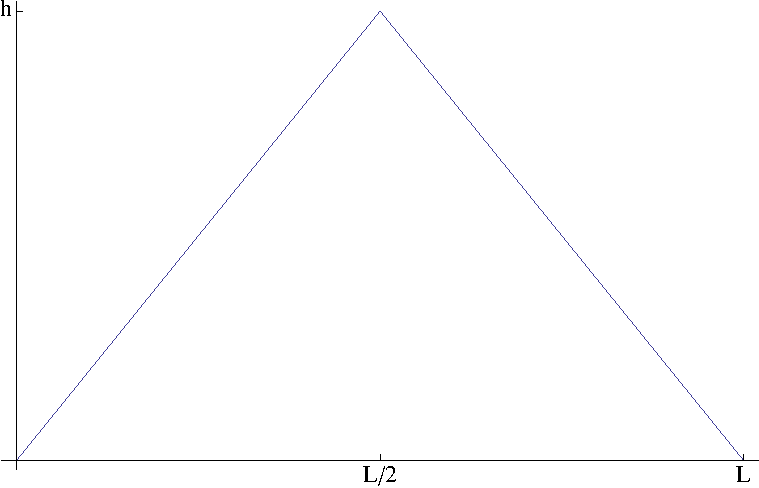
\includegraphics[scale=0.4]{string2.pdf}
  \end{minipage}
  \begin{minipage}{5cm}
$$y(x,0)=\left\{ 
\begin{array}{l l} 
  \frac{2 h}{L}x \mbox{ se } &  x<L/2 \\
  2 h -\frac{2 h}{L}x \mbox{ se } &  x>L/2
\end{array}
\right.
$$

$$\dot{y}(x,0)=0$$
 \end{minipage}
 \vspace{1 cm} }

\frame{\frametitle{Solução} Usando as condições iniciais temos que:

$$y(x,0)=\sum_{n=1}^\infty A_n \sin\left( \frac{n \pi x }{L} \right) \quad A_n=?$$

$$\dot{y}(x,0)= -\sum_{n=0}^\infty B_n \frac{n \pi c}{L} \sin\left( \frac{n \pi x }{L} \right)=0$$
$$B_n=0$$
}

\frame{\frametitle{Determinando $A_n$} Vamos usar a seguinte
  identidade:

$$\int_{0}^L \sin \left( \frac{n \pi x}{L} \right) \sin \left( \frac{m \pi x}{L} \right)\,dx=L/2\delta_{nm}$$

Usando a condição inicial:
$$\int_0^L y(x,0) \sin \left( \frac{m \pi x}{L} \right)=\int_{0}^L\sum_{n=1}^\infty A_n \sin\left( \frac{n \pi x }{L} 
\right) \sin \left( \frac{m \pi x}{L} \right)$$

$$\int_0^L y(x,0) \sin \left( \frac{m \pi x}{L} \right)=\frac{L A_m}{2}$$

$$A_m=\frac{2}{L}\int_0^L y(x,0) \sin \left( \frac{m \pi x}{L} \right)$$
}


\frame{\frametitle{Determinando $A_n$} Até agora esta solução é geral,
  particularizando para a nossa função. Temos:


$$A_m=\frac{2}{L}\int_0^{L/2} \frac{2 h x}{L} \sin \left( \frac{m \pi x}{L} \right) \,dx+
\int_{L/2}^L \left( 2h -\frac{2 h x}{L} \right) \sin \left( \frac{m
    \pi x}{L} \right) \,dx
$$

$$A_m=\left\{ 
\begin{array}{l l} 
  0 \mbox{ se } &  m \mbox{ é par}\\
  \frac{8 (-1)^{(m+1)/2}}{m^2 \pi ^2} \mbox{ se } &  m \mbox{ é impar}
\end{array}
\right.
$$

Use o resultado:
$$\int x\sin \left( \frac{m \pi x}{L} \right) \,dx=\frac{L^2 \sin \left(\frac{2 \pi  x}{L}\right)}{4 \pi ^2}-\frac{L x \cos \left(\frac{2
      \pi x}{L}\right)}{2 \pi }$$ }


\frame{\frametitle{Aproximação}

  Comparação entre a aproximação para 5 termos e o resultado esperado.
  \begin{center}
    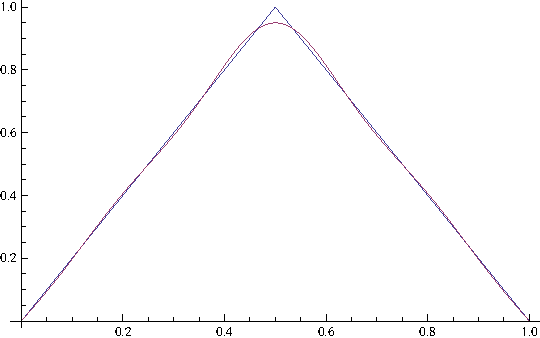
\includegraphics[scale=0.5]{fourier2.pdf}
  \end{center}

} \frame{\frametitle{Interpretação dos resultados}

  \begin{itemize}
  \item ``Qualquer'' função no intervalo $[0,L]$ pode ser representada
    como uma soma de senos e cossenos.
  \item Podemos considerar o espaço de todas as funções que podem ser
    expressas como a soma de senos e cossenos no intervalo $[0,L]$.
  \item Este espaço é vetorial. (Mostre!).
  \end{itemize}
}

\frame{\frametitle{Interpretação dos resultados}
  \begin{itemize}
  \item As funções
$$\sqrt{\frac{2}{L}} \sin \left( \frac{m \pi x}{L} \right) \quad \sqrt{\frac{2}{L}} \cos \left( \frac{m \pi x}{L} \right) $$
formam uma base ortonormal para esse espaço.
$$f(x)=\sum_{m=0}^\infty A_n\sqrt{\frac{2}{L}} \sin \left( \frac{m \pi x}{L} \right)+B_n\sqrt{\frac{2}{L}} \cos \left( \frac{m \pi x}{L} \right) $$
Note que:
$$\int_0^L \sqrt{\frac{2}{L}} \sin \left( \frac{m \pi x}{L} \right) \sqrt{\frac{2}{L}} \cos \left( \frac{n \pi x}{L} \right) =0$$
  \end{itemize}
}

\frame{\frametitle{Interpretação dos resultados} Considere duas
  funções $f$ e $g$. A integral:

$$\int_0^L f(x) g(x)\, dx$$

pode ser interpretada como um produto interno. Para se convencer disso
discretize a função e pense no vetor:
$$
( f(x_1),\ldots ,f(x_n))
$$
 }

\frame{\frametitle{Exercício} Considere a base formada pelos senos e
  cossenos, ignore o caso $n=0$.

  \begin{itemize}
  \item Escreva o operador paridade $P[f(x)]=f(-x)$.
  \item Escreva a representação matricial do operador derivada.
  \item Escreva a representação matricial do operador integral.
  \end{itemize}

  Ordene os vetores da base de uma forma conveniente.



}

\section{Problemas de Sturm Liouville}


\frame{\frametitle{Problemas de Sturm Liouville}

Equação característica para $\lambda$:

$$\frac{d}{dx}\left[ p(x) \frac{d y}{dx} \right] -s(x) y + \lambda r(x) y=0$$

$$x\in [a,b]$$
Operador linear:

$${\cal L}=\frac{d}{dx}\left[ p(x) \frac{d}{dx}\right] - s(x)$$

Autofunções e autovalores:

$y_m$ e $\lambda_m$
}

\frame{\frametitle{Problemas de Sturm Liouville}

Vamos demonstrar que as autofunções formam uma base ortogonal para as funções em $[a,b]$.
}

\frame{\frametitle{Problemas de Sturm Liouville}
$$\frac{d}{dx}\left[ p(x) \frac{d y_n}{dx} \right] -s(x) y_n + \lambda_n r(x) y_n=0$$
$$\frac{d}{dx}\left[ p(x) \frac{d y_m}{dx} \right] -s(x) y_m + \lambda_m r(x) y_m=0$$
Temos que:
$$y_n\frac{d}{dx}\left[ p(x) \frac{d y_m}{dx} \right] -s(x) y_ny_m + \lambda_n r(x) y_ny_m=0$$
$$y_m\frac{d}{dx}\left[ p(x) \frac{d y_n}{dx} \right] -s(x) y_ny_m + \lambda_n r(x) y_ny_m=0$$
Subtraindo as eqs. acima:
$$y_m\frac{d}{dx}\left[ p(x) \frac{d y_n}{dx} \right]-y_n\frac{d}{dx}\left[ p(x) \frac{d y_m}{dx} \right]$$
$$ =-(\lambda_m- \lambda_n) r(x) y_ny_m$$
}

\frame{\frametitle{Problemas de Sturm Liouville}

Integrando:

$$\int_a^b y_m\frac{d}{dx}\left[ p(x) \frac{d y_n}{dx} \right]-y_n\frac{d}{dx}\left[ p(x) \frac{d y_m}{dx} \right]\, dx =$$

$$=\int_a^b(-\lambda_m- \lambda_n) r(x) y_ny_m\, dx$$

Realizando a integração por partes:

$$\left\{ y_n p(x)\frac{d y_m}{d x}-y_m p(x)\frac{d y_n}{d x} \right\}_a^b-p(x)\frac{dy_m}{dx}\frac{dy_n}{dx}+p(x)\frac{dy_m}{dx}\frac{dy_n}{dx}$$

$$=-\int_a^b(\lambda_m- \lambda_n) r(x) y_ny_m\, dx$$

}

\frame{\frametitle{Problemas de Sturm Liouville}


$$\left\{ p(x)\left[ y_n \frac{d y_m}{d x}-y_m \frac{d y_n}{d x} \right]\right\}_a^b=-(\lambda_m- \lambda_n)\int_a^b r(x) y_ny_m\, dx$$

Assumindo $\lambda_n\neq\lambda_m$, para que tenhamos:
$$\int_a^b r(x) y_ny_m=0$$

Basta que:

\begin{itemize}
\item $y(a)=y(b)=0$ ou
\item $y^\prime (a)=y^\prime (b)=0$
\end{itemize}

Neste caso dizemos que as funções $y_m$ e $y_n$ são ortogonais com peso $r(x)$.
}

\frame{\frametitle{Problemas de Sturm Liouville}
Além disso:

$$f(x)=\sum_m a_m y_m(x)$$

$$\int_a^b f(x) r(x) y_n(x)=\sum_m\int_a^b y_my_n r(x)\, dx=a_n\int_a^by_m^2(x)r(x)\,dx$$

$$a_n=\frac{\int_a^b f(x) r(x) y_n(x) \, d x}{\int_a^b y_n^2(x) r(x) \, dx}$$
}

\frame{\frametitle{Membrana Circular}
$$\nabla^2u=\frac{1}{c^2}\frac{\partial^2 u}{\partial t^2}$$

$u(a)=0$

$u^\prime(r,\theta;0)=0$

$u(r,\theta;0)=f(r,\theta)$
}

\frame{\frametitle{Membrana Circular}
$$u(r,\theta,t)=\Lambda(r,\theta)T(t)=R(r)\Theta (\theta) T(t)$$

$$\nabla^2 u(r,\theta,t)=T\nabla^2\Lambda=\frac{1}{c^2}T^{\prime\prime}\Lambda (r,\theta)$$ 

$$\frac{T^{\prime\prime}}{T}=-\omega^2 \quad \frac{\nabla^2 \Lambda}{\Lambda}=-\frac{\omega^2}{c^2}$$

$$T=A \cos \omega t + B \sin \omega t $$
}

\frame{\frametitle{Parte Espacial}

$$\nabla^2\lambda=\left[
\frac{\partial^2}{\partial r^2}+\frac{1}{r}\frac{\partial^2}{\partial r}+ \frac{1}{r^2} 
\frac{\partial^2}{\partial \theta^2}
\right] R \Theta =-\frac{\omega^2}{c^2} R\Theta$$

$$\left[R^{\prime\prime}\Theta +\frac{1}{r}\Theta R +\frac{1}{r^2} R \Theta^{\prime\prime}\right] =-\frac{\omega^2}{c^2} R\Theta$$

$$\frac{\Theta^{\prime\prime}}{\Theta}=r^2\left[ 
-\frac{R^{\prime\prime}}{R}-\frac{1}{r}\frac{R^\prime}{R}-\frac{\omega^2}{c^2}\right]$$

}

\frame{\frametitle{Parte Angular}
$$\frac{\Theta^{\prime\prime}}{\Theta}=-\alpha^2$$ 

$$\Theta=A \sin \alpha \theta + B \cos \alpha \theta$$

Para que $\Theta$ seja periódica:

$\alpha=0,1,2,3\ldots $


}


\frame{\frametitle{Parte Radial}
$$-n^2 R = - r^2R^{\prime\prime} - r R^\prime -c^2 \omega^2 r^2 R$$

$$ r^2R^{\prime\prime} + r R^\prime +(c^2 \omega^2 r^2-n^2) R=0$$


Esta é a equação de Bessel. 
}

\frame{\frametitle{Equação de Bessel}
$$ r^2R^{\prime\prime} + r R^\prime +(k^2 r^2-n^2) R=0$$

$$x=kr$$

$$\frac{\partial R}{\partial r}=\frac{\partial R}{\partial x}\frac{\partial x}{\partial r}
=k\frac{\partial R}{\partial x}$$
}


\frame{\frametitle{Equação de Bessel}
$$x^2R^{\prime\prime}+xR^{\prime}+(x^2-n^2)R=0$$

Método das séries:

$$R(x)=\sum_{l=0}^\infty a_l x^{l+s}$$

$$\sum_{l=0}^\infty a_l (l+s)(l+s-1)x^{l+s}+\sum_{l=0}^\infty a_l(l+s)x^{l+s}+\sum_{l=0}^\infty a_lx^{l+s+2} +$$

$$\sum_{l=0}^\infty (-n^2)a_lx^{l+s}=0$$
}

\frame{\frametitle{Equação de Besse é SL}

$$\frac{d}{dx}\left[ p(x) \frac{d y}{dx} \right] -s(x) y + \lambda r(x) y=0$$

$$(r R^\prime)^\prime+(k^2r-n^2/r)R=0$$

$$p(x)=x\quad s(x)=-n^2/r \quad r(x)=r \quad \lambda=k^2$$

}

\frame{\frametitle{Equação de Bessel}
Drible da Vaca:

$$\sum_{l=0}^\infty a_l x^{l+s+2}=\sum_{l=2}^\infty a_{l-2} x^{l+s}$$

$$\sum_{l=2}^\infty [a_l(l+s)^2+a_{l-2}-n^2a_l]x^{l+s}+$$

$$[a_os^2-n^2a_o]x^s+[a_1(s+1)^2-n^2a_1]x^{s+1}=0$$

$$s^2=n^2\quad s=\pm n$$

}
\frame{\frametitle{Equação de Bessel $s=n$}

$$a_l=\frac{a_{l-2}}{n^2-(l+n)^2}=\frac{a_{l-2}}{n^2-n^2-2ln-l^2}$$

$$a_l=\frac{-a_{l-2}}{l(l+2n)}$$ 

$$a_1 [(n+1)^2-n^2]=a_1(2n +1)=0 \quad a_1=0$$
}

\frame{\frametitle{Equação de Bessel $s=n$}

$$a_{2k}=-\frac{a_{2(k-1)}}{2 k(2 k +2 n)}=\frac{-a_{2(k-1)}}{2^2 k(k+n)}$$

$$a_{2k}=\frac{(-1)^k}{2^{2k}k!(n+1)(n+2)\ldots (n+k)}$$

Padronização:

$$a_o=\frac{1}{2^n n!}\quad a_{2k}=\frac{(-1)^k}{2^{n+2k} k!(n+k)!}$$

$$J_n(x)=\sum_{l=0}^\infty \frac{(-1)^l x^{n+2l}}{2^{n+2l}(n+l)!l!}$$
}

\frame{\frametitle{Equação de Bessel $s=-n$}

$$a_l=\frac{-a_{l-2}}{n^2-(l^2-2ln+n^2)}=\frac{-a_{l-2}}{l(l-2 n)}$$

$$a_{2k}=\frac{-a_{2(k-1)}}{2^2k (k-n)}=\frac{(-1)^ka_0}{2^{2k}(-n).(-n+1)\ldots (-n+k)}$$

Problemas se $n$ é inteiro. Este caso deveria ser analisado com mais cuidado. Se procedessemos 
nesta direção iríamos obter as funções de von Neumann que não nos interessam pois estas divergem na origem.
}


\frame{\frametitle{Equação de Bessel}

\begin{center}
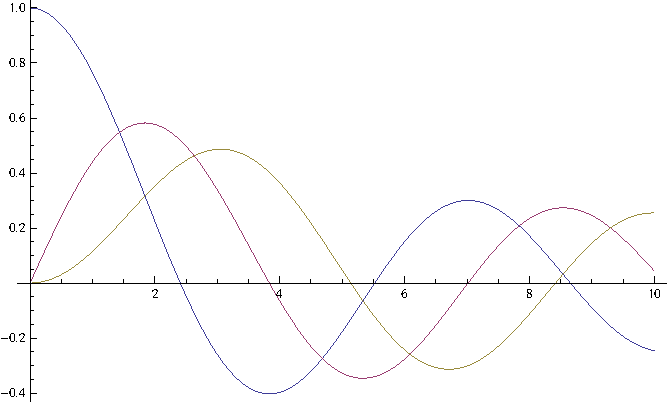
\includegraphics[scale=0.5]{bessel}
\end{center}
Lembrando que $x=kr$.

$R(a)=0\quad J_n(ka)=0$

$ka=\gamma_{n,m}$

m-ésima raiz da n-ésima função de Bessel.
}

\frame{\frametitle{Solução Geral}
$$\omega_{nm}=\frac{\gamma_{n,m}c}{a}$$

$$u(r,\theta ,t)=\sum_{n=0}^\infty \sum_{m=1}^\infty J_n\left( \frac{\gamma_{n,m}r}{a}\right)
(A_{nm}\cos (n\theta)+B_{nm}\sin (n\theta))$$
$$\times (C_{nm}\cos \omega_{nm}t +D_{nm}\sin (\omega_{nm} t))$$

}

\frame{\frametitle{Caso Particular}

$$u(r,\theta,0)=f(r,\theta)$$

$$\dot{u} (r,\theta,0)=0$$

$$f(r,\theta)=\sum_{n=0}^\infty \sum_{m=1}^\infty J_n\left( \frac{\gamma_{n,m}r}{a}\right)
(A_{nm}\sin (n\theta)+B_{nm}\cos (n\theta))$$



$$A_{nm}=\frac{2 \int_0^a\int_0^{2\pi}f(r,\theta) r J_n\left( \frac{\gamma_{n,m}r}{a} \right)\sin (k\theta )}
{\int_0^a r J^2_n\left( \frac{\gamma_{n,m}r}{a} \right)}$$

$$B_{nm}=\frac{2 \int_0^a\int_0^{2\pi}f(r,\theta) r J_n\left( \frac{\gamma_{n,m}r}{a} \right)\cos (k\theta )}
{\int_0^a r J^2_n\left( \frac{\gamma_{n,m}r}{a} \right)}$$
}

\frame{\frametitle{Exercício}
Considere $f(r,\theta )$ como sendo um cone de altura $h$ e raio $a$ centrado na origem. Considere apenas 
os 10 primeiros termos da expansão de Fourier generalizada.
}
\end{document}


